\begin{center}\textsc{Gauss} an \textsc{Olbers}.\quad Göttingen, 14. Mai 1826.\end{center}

.\ .\ .\ .\ .\ .\ Ich war beträchtliche Zeit mit der Ausgleichung meines
Winkelsystems beschäftigt. Weil ich jede Willkür ausschließen wollte, war
das eine sehr beschwerliche Arbeit, da dabei alles miteinander zusammenhängt
und sich die Messungen in Jever gewissermaßen auf die in Göttingen auswirken.
Vielleicht hat noch nie jemand eine so komplizierte Elimination ausgeführt,
bei der 55 Gleichungen ebenso viele Unbekannte enthielten. Heute bin ich
damit fertig geworden, sodass nun alle 150 Richtungen des Systems mit den
kleinstmöglichen Änderungen so ausgeglichen sind, dass sie genau miteinander
übereinstimmen. Unter den 150 sind fünf, die um mehr als $1^{\prime\prime}$ geändert
werden mussten (die größten Änderungen betragen $1^{\prime\prime}{,}373$, nämlich
Garlste-Varel und Varel-Garlste), und der sogenannte mittlere Richtungsfehler
beträgt $0^{\prime\prime}{,}755$, viel mehr, als die gute Übereinstimmung der
Messungen untereinander auf jeder Station zulässt. Daher kann ich an der
Existenz der Seitenrefraktion in den flachen Gegenden gar nicht zweifeln.
In den höheren Gegenden sind die Ausgleichungen immer viel kleiner. ---

Es war eine langweilige Arbeit, zunächst alle Messungen sorgfältig vorzubereiten,
da ich nichts vernachlässigen wollte und die kleinen Reduktionen der Konsequenz
halber überall berücksichtigt werden sollten. \textsc{Bessel} hat, soweit ich
weiß, zuerst öffentlich von der Reduktion gesprochen, die sich daraus ergibt,
dass sich der Winkel der kürzesten Linie vom Winkel der Vertikalebene
unterscheidet. Er hat dabei die Punkte nur auf der Oberfläche des Sphäroids betrachtet:
\clearpage
\noindent\textbf{ZUR NETZAUSGLEICHUNG.}\hfill321\par\medskip
\noindent Meistens beträgt diese Reduktion nur ein paar Tausendstel einer
Bogensekunde. Wollte ich sie aber einmal berücksichtigen, so durfte ich eine andere
nicht übergehen, die gewöhnlich viel größer (obgleich immer noch unbedeutend)
ist. Sie rührt daher, dass die Punkte, die auf ein und derselben Vertikallinie
liegen, nicht in ein und derselben Vertikalebene erscheinen, sodass sich eine
von der Höhe abhängige Reduktion ergibt. Sie hat immer das entgegengesetzte
Vorzeichen von \textsc{Bessels} Korrektur und ist schon bei mäßigen Höhen immer
größer, oft 4-mal oder 8-mal so groß, sodass jene immer aufgehoben und
weit übertroffen wird. Der größte Betrag in meinem System ergibt sich
von Lichtenberg zum Brocken, wo er $-0^{\prime\prime}{,}041$ ausmacht. ---
Die genaue Berechnung der 51 Dreiecke selbst wird jetzt ein Leichtes sein.
\par\medskip
.\ .\ .\ .\ .\ .

Ich habe mir heute noch etwas das System der \textsc{Krayenhoff}schen
Dreiecke im Inneren von Holland angesehen. Ich sehe immer mehr, wie wenig
Grund ich habe, mich über meinen größten Richtungsfehler von $1^{\prime\prime}{,}4$
zu beunruhigen. Wenn man \textsc{Krayenhoffs} Messungen oberflächlich prüft,
also die Summen der 3 Dreieckswinkel und den Horizontschluss, findet man
überall eine so gute Übereinstimmung, dass man versucht ist, diesen Messungen
eine Genauigkeit zuzuschreiben, von der sie doch \textls[120]{sehr} weit
entfernt sind. Nichts eignet sich für die Prüfung besser als die Verbindungen
von mehr als 3 Punkten, die miteinander verknüpfte Dreiecke ergeben. Hier
findet man häufig viel größere Abweichungen.
\begin{center}
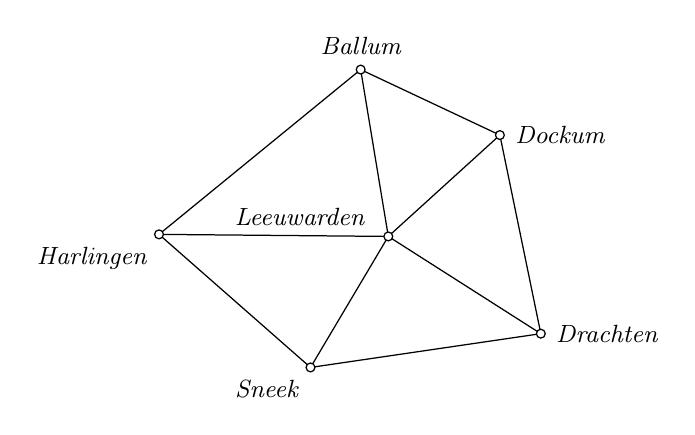
\begin{tikzpicture}[x=1.3cm,y=1.3cm,line width=.45pt,font=\small\itshape]
\coordinate (H) at (0,1.30);
\coordinate (B) at (1.97,2.91);
\coordinate (D) at (3.33,2.27);
\coordinate (R) at (3.73,.33);
\coordinate (S) at (1.48,0);
\coordinate (L) at (2.24,1.28);
\draw (H)--(B)--(D)--(R)--(S)--cycle;
\draw (L)--(H) (L)--(B) (L)--(D) (L)--(R) (L)--(S);
\foreach \p in {H,B,D,R,S,L}{\draw[fill=white] (\p) circle[radius=1.6pt];}
\node[above=2pt] at (B) {Ballum};
\node[right=2pt] at (D) {Dockum};
\node[right=2pt] at (R) {Drachten};
\node[below left=1pt] at (S) {Sneek};
\node[below left=1pt] at (H) {Harlingen};
\node[anchor=east,xshift=-.18cm,yshift=.25cm] at (L) {Leeuwarden};
\end{tikzpicture}
\end{center}
\begingroup
\makeatletter
\renewcommand{\@makefnmark}{\hbox{\normalfont[\textsuperscript{*})]}}
\renewcommand{\@makefntext}[1]{\parindent1em\noindent\hbox to1.8em{\hss[\textsuperscript{*})\ }#1]}
\makeatother
\noindent Zum Beispiel ergibt das System von 6 Punkten\footnote{Vgl. Band IV,
S.\ 82/87.} für Leeuwarden einen ausgezeichneten Horizontschluss, auf
$2^{\prime\prime}{,}197$ genau. Die Winkelsummen in den 5 Dreiecken weichen
jeweils ab um
\[
\begin{array}{r}
1^{\prime\prime}{,}432\\
0{,}714\\
0{,}759\\
2{,}842\\
2{,}590,
\end{array}
\]
\endgroup
\makeatletter
\def\ps@gaussIXfortyone{\def\@oddhead{}\def\@evenhead{}\def\@oddfoot{\small IX.\hfil41}\let\@evenfoot\@oddfoot}
\makeatother
\thispagestyle{gaussIXfortyone}
\clearpage
\noindent322\hfill\textbf{BRIEFWECHSEL.}\par\medskip
\begingroup
\makeatletter
\renewcommand{\@makefnmark}{\hbox{\normalfont\textsuperscript{*})}}
\makeatother
\noindent also auch noch erträglich. Prüft man aber die Seitenverhältnisse,
so zeigt sich, dass sich die Messungen nur durch viel größere Änderungen an
den 10 Winkeln am Rand in Einklang bringen lassen. Nach der Methode der
kleinsten Quadrate müsste man sie um
$3^{\prime\prime}{,}8$, $3^{\prime\prime}{,}6$, $3^{\prime\prime}{,}6$, $3^{\prime\prime}{,}3$, $3^{\prime\prime}{,}0$, $2^{\prime\prime}{,}7$, $2^{\prime\prime}{,}7$,
$1^{\prime\prime}{,}9$, $1^{\prime\prime}{,}1$, $0^{\prime\prime}{,}8$ ändern.
Wollte man die Änderungen so klein wie möglich halten, so müsste man sie
alle 10 gleich und jede $=3^{\prime\prime}$ setzen\footnote{\textsc{Krayenhoffs} eigene Ausgleichung, die aber nicht klar dargestellt ist, sondern erst herausgesucht werden muss, enthält hier zum Teil noch viel größere Änderungen, z.\ B.\ von $6^{\prime\prime}{,}253$ an dem einen Winkel in Drachten, $5^{\prime\prime}{,}530$ an einem Winkel in Dockum usw.}.
Man sieht also, dass bei solchen Messungen die Summe der 3 Dreieckswinkel oft
um mehr als $10^{\prime\prime}$ abweichen müsste. Davon sind die angegebenen
Zahlen aber weit entfernt, und somit [ist] gewiss, dass zumindest stets nur
so \textls[120]{ausgewählt} wurde, dass \textls[120]{diese} Prüfung aufgeht.
Dadurch müssen die Winkel aber offenbar oft eher verschlechtert als
verbessert werden, und es ergibt sich ein ganz falscher Maßstab für ihre
Genauigkeit. Um die Genauigkeit von Messungen angemessen beurteilen zu können,
darf nichts willkürlich ausgeschlossen werden. Die einfachen Prüfungen
anhand der Summen der 3 Dreieckswinkel und des Horizontschlusses sind wohl
allzu verführerisch, wenn auch nicht gerade zum Verfälschen, so doch zum
Auswählen und Ausschließen, was kaum besser ist. Leider lassen andere
Messungen, wie die von \textsc{Delambre}, außer den erwähnten fast keine
Prüfungen zu. Sonst würde man wohl oft ähnliche Abweichungen finden.

Bei meinem System hatte ich die Genugtuung, dass die Prüfungen beider
Arten Abweichungen von ganz derselben Größenordnung ergeben. Dass
Seitenrefraktionen so große Auswirkungen haben wie die Abweichungen in
\textsc{Krayenhoffs} Dreiecken, bezweifle ich allerdings, da seine Seiten
immer so kurz sind, seine Stationen hoch in der Luft liegen und Holland
wohl auch viel weniger durch Wald unterteilt ist als mein nördliches Gelände.
Bei ihm ist das Licht daher wohl selten oder nie so knapp an Hindernissen
vorbeigegangen, wie es im letzteren so häufig geschah. Ich würde die
Anomalien deshalb eher den Messungen selbst zuschreiben.
\endgroup
